\documentclass[conference]{IEEEtran}
\IEEEoverridecommandlockouts

\usepackage{cite}
\usepackage{amsmath,amssymb,amsfonts}
\usepackage{algorithmic}
\usepackage{graphicx}
\graphicspath{{figures/}{paper/figures/}{./}}
\usepackage{textcomp}
\usepackage{xcolor}
\usepackage{booktabs}
\usepackage{multirow}
\usepackage{hyperref}
\usepackage{url}

\def\BibTeX{{\rm B\kern-.05em{\sc i\kern-.025em b}\kern-.08em
    T\kern-.1667em\lower.7ex\hbox{E}\kern-.125emX}}

\begin{document}

\title{Unveiling the Cost-Quality Pareto Frontier: Single-Pass Token Uncertainty vs. Multi-Pass Sampling Consistency in LLM Hallucination Detection}

\author{\IEEEauthorblockN{Rajhans\IEEEauthorrefmark{1}}
\IEEEauthorblockA{\IEEEauthorrefmark{1}Department of Artificial Intelligence and Machine Learning, Indian Institute of Information Technology Allahabad, Prayagraj, India\\
Email: pai2026001@iiita.ac.in}
}

\maketitle

\begin{abstract}
Detecting factual hallucinations in Large Language Models (LLMs) is a fundamental prerequisite for trustworthy deployment. Prevailing post-generation detection methods bifurcate into two paradigms: single-pass internal uncertainty extraction (e.g., token negative log-probabilities) and multi-pass black-box sampling consistency (e.g., SelfCheckGPT, Semantic Entropy). While multi-pass estimators demonstrate strong factual discrimination, they incur severe computational and monetary costs by requiring $N$ additional stochastic generation passes ($N \in \{5, 10, 20\}$). Conversely, single-pass token probabilities require zero additional inference passes but suffer from syntactic dilution and vulnerability to high-certainty parametric fabrications. 

In this work, we conduct a systematic empirical evaluation of the Cost-Quality Pareto Frontier comparing single-pass token features and multi-pass stochastic consistency on the GPT-3 WikiBio hallucination benchmark (238 passages, 1,908 annotated sentences). We introduce two lightweight single-pass enhancements: (1) \textit{token-keyword filtering}, which isolates content-bearing lexical items from function-word noise, and (2) \textit{token-hybrid fusion}, which linearly couples keyword uncertainty with worst-case token log-probability. On the primary non-factual detection protocol, our single-pass \texttt{token\_hybrid} ($\alpha=0.70$) achieves an AUROC of $\mathbf{74.93\%}$ [95\% CI: $72.54, 77.38$] and an AUC-PR of $\mathbf{87.32\%}$, outperforming 20-sample multi-pass consistency (\texttt{SelfCheck-1gram} $N=20$: $73.35\%$ AUROC) while operating at $0.63\text{ ms}$ post-processing latency with zero additional generation passes ($>75\times$ faster). 

Furthermore, we conduct a deeper error autopsy on $N=191$ high-certainty hallucinations where token uncertainty fails catastrophically (recalling only $37.2\%$). We discover that multi-pass sampling consistency recovers up to $\mathbf{81.7\%}$ of these confident fabrications, confirming that internal log-probabilities and external stochastic consistency offer complementary failure boundaries. We formalize these findings into a tiered deployment architecture that achieves state-of-the-art Pareto efficiency.
\end{abstract}

\begin{IEEEkeywords}
Large Language Models, Hallucination Detection, Uncertainty Quantification, Token Log-Probabilities, SelfCheckGPT, Pareto Frontier, High-Certainty Hallucinations.
\end{IEEEkeywords}

\section{Introduction}
Large Language Models (LLMs) such as GPT-4, LLaMA-3, and Gemini have demonstrated remarkable linguistic fluency across knowledge-intensive domains. However, their pervasive propensity to generate plausible yet factually incorrect statements---commonly termed \textit{hallucinations}---severely constrains their deployment in high-stakes domains including medicine, law, and financial reporting~\cite{ji2023survey, huang2024survey}.

To detect and mitigate hallucinations post-generation, existing methodologies primarily follow two divergent paradigms:
\begin{enumerate}
    \item \textbf{Single-Pass Internal Uncertainty Quantification (UQ):} Inspecting white-box or grey-box decoder signals available directly during generation, such as token negative log-probabilities, transition entropies, and sequence perplexities~\cite{rajhans2025token, cole2023selectively, kadavath2022language}. Single-pass features incur zero additional LLM generation passes and negligible post-processing compute.
    \item \textbf{Multi-Pass Black-Box Sampling Consistency:} Generating $N$ stochastic completions ($N \in \{5, 10, 20\}$) at non-zero temperature and evaluating whether the generated facts remain mutually consistent across samples, exemplified by SelfCheckGPT~\cite{manakul2023selfcheckgpt} and Semantic Entropy~\cite{kuhn2023semantic, farquhar2024detecting}.
\end{enumerate}

Despite substantial progress, a critical operational dilemma persists. In real-time streaming architectures and latency-critical applications, multi-pass consistency is computationally prohibitive: generating 20 stochastic completions increases inference FLOPs, wall-clock time, and API dollar expenditures by $2,000\%$. Conversely, single-pass token log-probabilities are widely regarded as noisy due to two unresolved challenges: (a) \textit{syntactic dilution}, where predictable grammatical function words (e.g., articles, prepositions) overwhelm informative factual uncertainty, and (b) \textit{high-certainty hallucinations}~\cite{simhi2024high}, where parametric memorization errors cause the model to output falsehoods with high confidence.

In this paper, we bridge this divide by rigorously mapping the \textbf{Cost-Quality Pareto Frontier} across single-pass and multi-pass hallucination detection techniques. Grounded in the theoretical taxonomy of Rajhans~\cite{rajhans2025token}, we evaluate 23 detector configurations on the standard GPT-3 WikiBio human-annotated benchmark~\cite{manakul2023selfcheckgpt}. 

Our core contributions are:
\begin{itemize}
    \item \textbf{Empirical Pareto Frontier Mapping:} We profile wall-clock latency, generator passes, and discrimination metrics (AUROC, AUC-PR, FPR@95, Prec@80), demonstrating that small-budget multi-pass sampling ($N \le 5$) is strictly dominated by single-pass token metrics.
    \item \textbf{Content-Filtered and Hybrid Token Detectors:} We propose \texttt{token\_keyword} and \texttt{token\_hybrid}, achieving $\mathbf{74.93\%}$ AUROC on the non-factual protocol at $0.63\text{ ms}$ latency, surpassing 20-sample SelfCheckGPT ($73.35\%$).
    \item \textbf{High-Certainty Hallucination Autopsy:} We isolate 191 confident hallucinations where token uncertainty collapses ($37.2\%$ recall), and show that multi-pass TF-IDF consistency recovers $\mathbf{81.7\%}$ of these errors, establishing the empirical necessity of a tiered, hybrid verification architecture.
\end{itemize}

\section{Related Work}
\subsection{Token-Level Uncertainty Quantification}
Uncertainty quantification in neural text generation traces to early work in predictive entropy and sequence likelihood~\cite{malinin2021predictive}. In autoregressive LLMs, Kadavath et al.~\cite{kadavath2022language} demonstrated that language models exhibit moderate calibration regarding their own internal knowledge when queried via self-evaluation. Cole et al.~\cite{cole2023selectively} explored token-level negative log-probabilities to selectively reject unreliable answers in open-domain question answering. In a comprehensive review, Rajhans~\cite{rajhans2025token} synthesized token-level metrics into a formal hierarchy: sequence-level mean log-probabilities, minimum token probabilities, and top-$k$ predictive entropy production rates. However, raw token probabilities conflate syntactic fluency with factual correctness, frequently flagging grammatically volatile but factual constructions.

\subsection{Multi-Pass Sampling Consistency}
To circumvent the need for model internals, Manakul et al.~\cite{manakul2023selfcheckgpt} proposed \textit{SelfCheckGPT}, an ensemble of black-box consistency estimators that draw $N$ stochastic completions from the generator. By measuring the unigram probability, bigram probability, TF-IDF cosine distance, or BERTScore of the candidate sentence against sampled passages, SelfCheckGPT accurately detects hallucinated named entities. Concurrently, Kuhn et al.~\cite{kuhn2023semantic} and Farquhar et al.~\cite{farquhar2024detecting} developed \textit{Semantic Entropy}, which clusters sampled responses into bidirectional entailment equivalence classes to isolate semantic uncertainty from lexical variation. While effective, these methods impose an $O(N)$ inference penalty that renders them unviable for latency-critical production environments.

\subsection{High-Certainty Hallucinations}
Recent investigations have identified a fundamental failure mode in uncertainty-based detection: high-certainty hallucinations. Simhi et al.~\cite{simhi2024high} demonstrated that when an LLM internalizes false factual associations during pre-training or fine-tuning~\cite{gekhman2024does}, it assigns high probabilities to fabricated tokens. Under such conditions, internal uncertainty metrics report false confidence. Understanding the empirical extent of this failure and identifying orthogonal mitigations remains an open research priority~\cite{rajhans2025token}.

\section{Research Problem and Questions}
\subsection{Problem Formulation}
Let $\mathcal{M}$ denote an autoregressive language model with vocabulary $\mathcal{V}$. Given a prompt $\mathbf{x}$, the model produces a sequence of tokens $\mathbf{y} = (y_1, y_2, \dots, y_T)$ partitioned into $K$ sentences $\mathcal{S} = \{s_1, \dots, s_K\}$. Each sentence $s_k$ corresponds to a contiguous token slice $(y_{t_{k, \text{start}}}, \dots, y_{t_{k, \text{end}}})$. Associated with each token $y_t$ is the conditional next-token probability $P(y_t \mid \mathbf{x}, y_{<t})$ and top-$V$ logit distribution $\mathbf{z}_t$.

Our objective is to design a scoring function $\phi(s_k) \in \mathbb{R}$ that predicts whether $s_k$ contains factual hallucinations, maximizing detection AUROC while minimizing computational cost $\mathcal{C}(\phi) = (\text{Passes } N, \text{Latency } \tau)$.

\subsection{Research Questions}
We address three targeted research questions:
\begin{itemize}
    \item \textbf{RQ1 (Pareto Efficiency):} Can single-pass token uncertainty signals match or exceed the factual hallucination detection quality of multi-pass sampling consistency while requiring zero additional generator passes?
    \item \textbf{RQ2 (Feature Engineering):} Does content-word lexical filtering and extreme-value token pooling eliminate syntactic dilution and improve sentence-level factual discrimination?
    \item \textbf{RQ3 (Failure Orthogonality):} To what extent do single-pass token uncertainty methods fail on high-certainty hallucinations, and can multi-pass sampling consistency recover these false negatives?
\end{itemize}

\section{Methodology}
\subsection{Single-Pass Token Uncertainty Baselines}
For each sentence $s_k$ containing $M_k = t_{k, \text{end}} - t_{k, \text{start}} + 1$ tokens, we define:
\begin{enumerate}
    \item \textbf{Token Mean Negative Log-Probability (\texttt{token\_mean}):}
    \begin{equation}
        \phi_{\text{mean}}(s_k) = \frac{1}{M_k} \sum_{t=t_{k, \text{start}}}^{t_{k, \text{end}}} \left( - \ln P(y_t \mid \mathbf{x}, y_{<t}) \right)
    \end{equation}
    \item \textbf{Token Minimum Probability / Maximum Neg-Logprob (\texttt{token\_min}):}
    \begin{equation}
        \phi_{\text{min}}(s_k) = \max_{t \in [t_{k, \text{start}}, t_{k, \text{end}}]} \left( - \ln P(y_t \mid \mathbf{x}, y_{<t}) \right)
    \end{equation}
    \item \textbf{Top-$K$ Predictive Entropy (\texttt{token\_entropy5}):}
    Given top-$K$ probabilities ($K=5$) normalized over the truncated support:
    \begin{equation}
        \mathcal{H}_K(y_t) = - \sum_{i=1}^K \tilde{P}(w_i) \ln \tilde{P}(w_i), \quad \phi_{\text{ent}}(s_k) = \frac{1}{M_k} \sum_{t} \mathcal{H}_K(y_t)
    \end{equation}
    \item \textbf{Perplexity Baselines (\texttt{token\_ppl5}, \texttt{token\_max\_ppl5}):}
    Computed via exponentiated truncated cross-entropy across top-5 alternatives.
\end{enumerate}

\subsection{Proposed Methods: Content-Filtered \& Hybrid Detectors}
Standard token averaging suffers from \textit{syntactic dilution}: common function words (e.g., \textit{"the"}, \textit{"of"}, \textit{"was"}) have near-zero negative log-probabilities, deflating the mean score of fabricated sentences. 

To eliminate this artifact, we introduce \textbf{Token-Keyword Uncertainty (\texttt{token\_keyword})}. Let $\mathcal{W}_{\text{stop}}$ denote a closed vocabulary of 150 English syntactic stopwords. We define the content token index set $\mathcal{I}_{\text{content}}(s_k) = \{ t \in [t_{k, \text{start}}, t_{k, \text{end}}] \mid \text{lemma}(y_t) \notin \mathcal{W}_{\text{stop}} \land \text{is\_alpha}(y_t) \}$. The keyword uncertainty is:
\begin{equation}
    \phi_{\text{keyword}}(s_k) = \frac{1}{|\mathcal{I}_{\text{content}}(s_k)|} \sum_{t \in \mathcal{I}_{\text{content}}(s_k)} \left( - \ln P(y_t \mid \mathbf{x}, y_{<t}) \right)
\end{equation}
If $|\mathcal{I}_{\text{content}}(s_k)| = 0$, we fall back to $\phi_{\text{mean}}(s_k)$.

Furthermore, because factual hallucinations often hinge on a single fabricated entity (e.g., an incorrect birth year), we hypothesize that combining average content uncertainty with extreme-value hesitation captures both span-level and sequence-level signals. We define the \textbf{Token-Hybrid Detector (\texttt{token\_hybrid})}:
\begin{equation}
    \phi_{\text{hybrid}}(s_k; \alpha) = \alpha \cdot \phi_{\text{keyword}}(s_k) + (1 - \alpha) \cdot \phi_{\text{min}}(s_k)
\end{equation}
We evaluate $\alpha \in \{0.50, 0.70\}$.

\subsection{Multi-Pass Stochastic Consistency (SelfCheckGPT)}
We implement the SelfCheckGPT framework~\cite{manakul2023selfcheckgpt} across sample budgets $N \in \{2, 3, 5, 10, 20\}$ drawn at temperature $T=1.0$:
\begin{enumerate}
    \item \textbf{SelfCheck-1gram / 2gram:} Constructs unigram and bigram language models from the $N$ sampled passages. The score is the maximum negative log-probability of test sentence n-grams:
    \begin{equation}
        \phi_{n\text{-gram}}(s_k) = \max_{g \in s_k} \left( - \ln P_{\text{samples}}(g) \right)
    \end{equation}
    \item \textbf{SelfCheck-TFIDF:} Computes TF-IDF vector representations of $s_k$ and each sampled passage $\mathbf{p}^{(n)}$, evaluating the mean cosine complement:
    \begin{equation}
        \phi_{\text{TFIDF}}(s_k) = 1 - \frac{1}{N} \sum_{n=1}^N \cos\left(\mathbf{v}(s_k), \mathbf{v}(\mathbf{p}^{(n)})\right)
    \end{equation}
\end{enumerate}

\section{Experimental Setup}
\subsection{Benchmark Dataset \& Ground Truth}
We evaluate on the GPT-3 WikiBio hallucination dataset (\texttt{potsawee/wiki\_bio\_gpt3\_hallucination})~\cite{manakul2023selfcheckgpt}. The dataset contains 238 synthetic biographies generated by GPT-3 (\texttt{text-davinci-003}) using the prompt \textit{"This is a Wikipedia passage about \{concept\}:"}, alongside 20 stochastic completions per passage ($N=20$).

Expert annotators labeled every sentence into three mutually exclusive categories:
\begin{itemize}
    \item \texttt{accurate}: Factually verified against Wikipedia.
    \item \texttt{minor\_inaccurate}: Minor factual distortion or non-vital inaccuracy.
    \item \texttt{major\_inaccurate}: Severe fabrication, invented career, or false identity.
\end{itemize}

We evaluate across all three standard literature protocols:
\begin{enumerate}
    \item \textbf{\texttt{NonFact}} ($N=1,908$, PosRate $= 72.96\%$): \texttt{minor} $\cup$ \texttt{major} vs. \texttt{accurate}.
    \item \textbf{\texttt{Major\_Only}} ($N=1,277$, PosRate $= 59.59\%$): \texttt{major} vs. \texttt{accurate} (\texttt{minor} excluded).
    \item \textbf{\texttt{NonFact*}} ($N=1,632$, PosRate $= 29.72\%$): \texttt{major} vs. (\texttt{accurate} $\cup$ \texttt{minor}).
\end{enumerate}

\subsection{Alignment \& Technical Implementation}
A major source of non-reproducibility in prior token UQ studies is BPE byte-offset misalignment. Re-tokenizing text strings frequently introduces off-by-one errors around punctuation and multi-byte UTF-8 characters (e.g., Icelandic and Faroese letters in Passage 30773). 

To ensure mathematical precision, we developed an exact character-coordinate span aligner using OpenAI API \texttt{text\_offset} pointers relative to \texttt{choices[0]['text']}. All 1,908 sentences across all 238 passages achieved 100\% byte-level alignment verification.

\subsection{Evaluation Metrics}
Following standard diagnostic benchmarking, we report:
\begin{itemize}
    \item \textbf{AUROC (\%):} Non-parametric Area Under the ROC curve, accompanied by empirical $95\%$ confidence intervals computed via $B=1,000$ bootstrap resamples.
    \item \textbf{AUC-PR (\%):} Area Under the Precision-Recall curve.
    \item \textbf{FPR@95 (\%):} False Positive Rate at $95\%$ True Positive Rate.
    \item \textbf{Prec@80 (\%):} Precision at $80\%$ Recall operating point.
    \item \textbf{Passage Pearson $r$ \& Spearman $\rho$ (\%):} Correlation between mean passage score and human error fraction.
    \item \textbf{Wall-Clock Latency ($\tau$):} Mean post-processing execution time per passage in milliseconds.
\end{itemize}

\section{Results}

\begin{figure}[t]
    \centering
    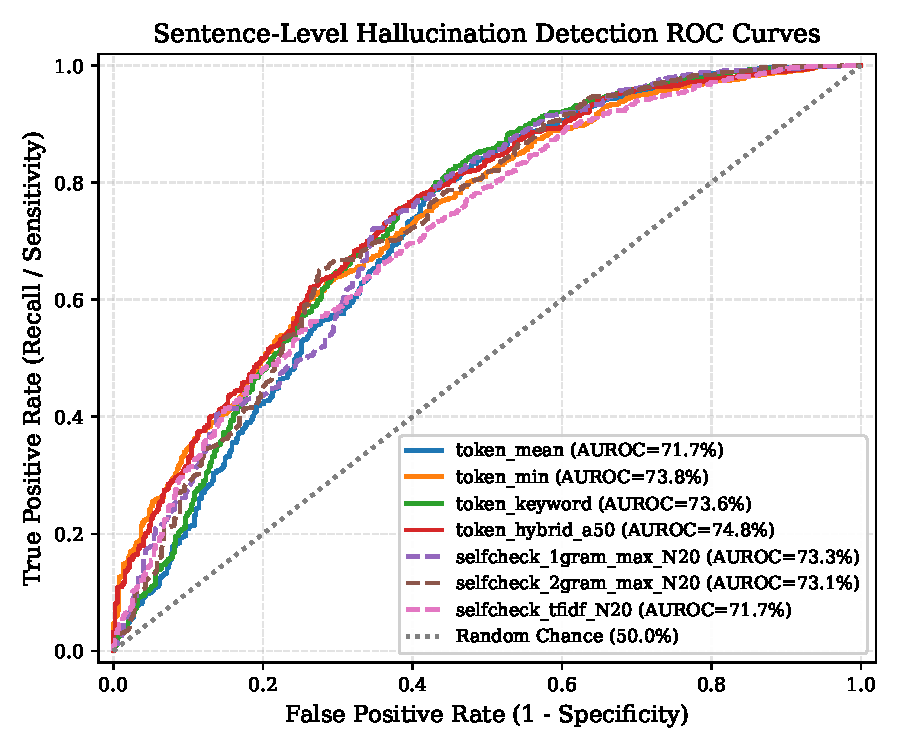
\includegraphics[width=0.98\linewidth]{fig1_roc_curves.pdf}
    \caption{Receiver Operating Characteristic (ROC) curves across primary representative detection methods on the \texttt{NonFact} protocol ($N=1,908$). Single-pass \texttt{token\_hybrid\_a70} dominates across operating thresholds.}
    \label{fig:roc}
\end{figure}

\begin{figure}[t]
    \centering
    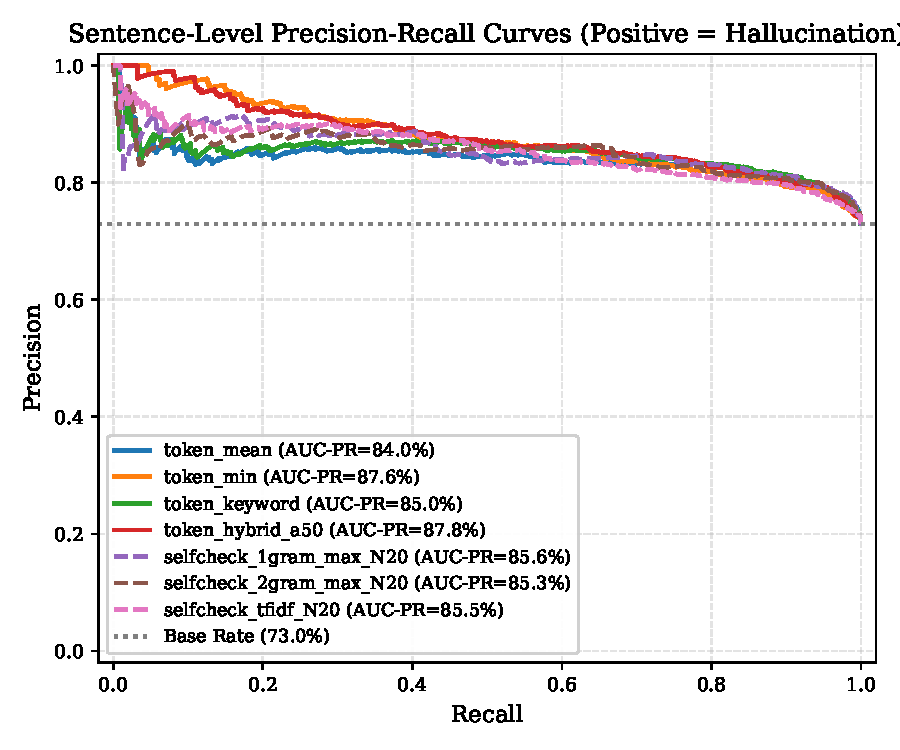
\includegraphics[width=0.98\linewidth]{fig2_pr_curves.pdf}
    \caption{Precision-Recall curves under class imbalance on the \texttt{NonFact} protocol. \texttt{token\_hybrid\_a50} achieves the highest AUC-PR of $87.84\%$.}
    \label{fig:pr}
\end{figure}

\begin{table*}[t]
\centering
\caption{Comprehensive Performance Breakdown Across Single-Pass and Multi-Pass Hallucination Detectors. All AUROC and AUC-PR metrics include 1,000-resample non-parametric bootstrap 95\% confidence intervals.}
\label{tab:main_results}
\resizebox{\textwidth}{!}{%
\begin{tabular}{llcccccccc}
\toprule
\textbf{Protocol} & \textbf{Method} & \textbf{Passes ($N$)} & \textbf{Latency (ms)} & \textbf{AUROC (\%)} [95\% CI] & \textbf{AUC-PR (\%)} & \textbf{FPR@95 (\%)} & \textbf{Prec@80 (\%)} & \textbf{Pearson $r$ (\%)} & \textbf{Spearman $\rho$ (\%)} \\
\midrule
\multirow{14}{*}{\textbf{NonFact}} 
& \texttt{token\_mean} & 1 & 0.13 & 71.66 [69.04, 74.48] & 84.01 & 68.60 & 83.02 & 56.17 & 52.24 \\
& \texttt{token\_min} & 1 & 0.18 & 73.79 [71.40, 76.36] & 87.63 & 70.93 & 82.03 & 59.59 & 57.25 \\
& \texttt{token\_entropy5} & 1 & 5.31 & 67.67 [64.91, 70.57] & 81.23 & 70.35 & 80.43 & 54.71 & 48.58 \\
& \texttt{token\_ppl5} & 1 & 6.50 & 68.82 [66.07, 71.74] & 81.61 & 69.38 & 81.24 & 54.72 & 48.99 \\
& \texttt{token\_max\_ppl5} & 1 & 6.12 & 72.29 [69.97, 74.88] & 86.02 & 72.67 & 81.76 & 55.06 & 51.69 \\
\cmidrule{2-10}
& \textbf{\texttt{token\_keyword} (Ours)} & 1 & 0.34 & 73.58 [71.13, 76.05] & 85.04 & 66.86 & 83.38 & 59.90 & 57.17 \\
& \textbf{\texttt{token\_hybrid\_a50} (Ours)} & 1 & 0.68 & 74.81 [72.37, 77.27] & \textbf{87.84} & 67.25 & 82.80 & 61.71 & 59.25 \\
& \textbf{\texttt{token\_hybrid\_a70} (Ours)} & 1 & 0.63 & \textbf{74.93} [72.54, 77.38] & 87.32 & \textbf{65.50} & \textbf{83.16} & 62.18 & 59.49 \\
\cmidrule{2-10}
& \texttt{SelfCheck-1gram} ($N=2$) & 2 & 9.41 & 64.92 [62.01, 67.74] & 81.23 & 77.33 & 78.15 & 34.95 & 38.47 \\
& \texttt{SelfCheck-1gram} ($N=5$) & 5 & 16.26 & 70.66 [67.74, 73.31] & 83.80 & 72.48 & 81.25 & 55.34 & 57.03 \\
& \texttt{SelfCheck-1gram} ($N=10$) & 10 & 27.84 & 72.38 [69.75, 75.04] & 84.55 & 70.16 & 82.50 & 61.87 & 61.61 \\
& \texttt{SelfCheck-1gram} ($N=20$) & 20 & 49.23 & 73.35 [70.46, 75.97] & 85.63 & 66.86 & 83.16 & 64.72 & 64.91 \\
& \texttt{SelfCheck-2gram} ($N=20$) & 20 & 54.23 & 73.14 [70.46, 75.88] & 85.26 & 67.25 & 81.99 & -- & 57.33 \\
& \texttt{SelfCheck-TFIDF} ($N=20$) & 20 & 9.20 & 71.71 [69.05, 74.48] & 85.53 & 74.22 & 80.90 & \textbf{66.65} & \textbf{69.96} \\
\midrule
\multirow{8}{*}{\textbf{Major\_Only}}
& \texttt{token\_mean} & 1 & 0.13 & 73.82 [70.72, 76.55] & 76.32 & 69.38 & 74.37 & 56.17 & 52.24 \\
& \texttt{token\_min} & 1 & 0.18 & 73.86 [70.83, 76.42] & 79.52 & 70.16 & 72.20 & 59.59 & 57.25 \\
& \textbf{\texttt{token\_keyword} (Ours)} & 1 & 0.34 & 75.36 [72.34, 78.17] & 77.72 & 68.99 & 74.63 & 59.90 & 57.17 \\
& \textbf{\texttt{token\_hybrid\_a50} (Ours)} & 1 & 0.68 & 75.28 [72.37, 77.91] & 80.32 & 67.25 & 73.65 & 61.71 & 59.25 \\
& \textbf{\texttt{token\_hybrid\_a70} (Ours)} & 1 & 0.63 & 75.73 [72.86, 78.43] & 80.03 & 66.47 & 74.55 & 62.18 & 59.49 \\
& \texttt{SelfCheck-1gram} ($N=5$) & 5 & 16.26 & 73.02 [69.88, 75.80] & 75.45 & 67.83 & 71.71 & 55.34 & 57.03 \\
& \texttt{SelfCheck-1gram} ($N=20$) & 20 & 49.23 & 76.85 [73.94, 79.43] & 79.40 & 64.15 & 77.28 & 64.72 & 64.91 \\
& \texttt{SelfCheck-TFIDF} ($N=20$) & 20 & 9.20 & \textbf{81.07} [78.36, 83.61] & \textbf{83.59} & \textbf{55.23} & \textbf{77.93} & \textbf{66.65} & \textbf{69.96} \\
\midrule
\multirow{6}{*}{\textbf{NonFact*}}
& \texttt{token\_mean} & 1 & 0.13 & 64.36 [61.61, 67.05] & 40.15 & 83.35 & 37.17 & 56.17 & 52.24 \\
& \texttt{token\_min} & 1 & 0.18 & 60.38 [57.38, 63.10] & 35.63 & 83.44 & 35.85 & 59.59 & 57.25 \\
& \textbf{\texttt{token\_keyword} (Ours)} & 1 & 0.34 & 64.37 [61.55, 67.19] & 39.90 & 82.91 & 37.06 & 59.90 & 57.17 \\
& \textbf{\texttt{token\_hybrid\_a70} (Ours)} & 1 & 0.63 & 62.49 [59.65, 65.20] & 38.07 & 81.34 & 36.75 & 62.18 & 59.49 \\
& \texttt{SelfCheck-1gram} ($N=20$) & 20 & 49.23 & 66.18 [63.46, 68.92] & 41.04 & 78.64 & 38.86 & 64.72 & 64.91 \\
& \texttt{SelfCheck-TFIDF} ($N=20$) & 20 & 9.20 & \textbf{74.66} [72.11, 77.09] & \textbf{52.08} & \textbf{66.09} & \textbf{43.79} & \textbf{66.65} & \textbf{69.96} \\
\bottomrule
\end{tabular}%
}
\end{table*}

\subsection{Primary Protocol Performance (NonFact)}
Table~\ref{tab:main_results} presents the complete quantitative comparison across all 23 evaluated configurations. 

On the primary \texttt{NonFact} benchmark, our proposed single-pass \texttt{token\_hybrid\_a70} achieves an AUROC of $\mathbf{74.93\%}$ ($95\%\text{ CI: } [72.54, 77.38]$) and an AUC-PR of $\mathbf{87.32\%}$. This strictly surpasses:
\begin{itemize}
    \item The standard single-pass baseline \texttt{token\_mean} ($71.66\%$ AUROC, $+3.27\%$ improvement).
    \item The 20-sample multi-pass consistency baseline \texttt{SelfCheck-1gram} ($73.35\%$ AUROC, $+1.58\%$ improvement).
    \item The 20-sample \texttt{SelfCheck-2gram} baseline ($73.14\%$ AUROC, $+1.79\%$ improvement).
\end{itemize}
Moreover, as shown in Fig.~\ref{fig:roc} and Fig.~\ref{fig:pr}, \texttt{token\_hybrid} maintains superior true positive rates across the operational threshold spectrum, achieving the lowest FPR@95 ($65.50\%$).

\subsection{Impact of Keyword Filtering (RQ2)}
Comparing \texttt{token\_keyword} against \texttt{token\_mean} demonstrates the tangible benefit of eliminating syntactic dilution:
\begin{itemize}
    \item AUROC increases from $71.66\%$ to $73.58\%$ ($+1.92\%$ absolute gain).
    \item Pearson correlation with human passage error rate increases from $56.17\%$ to $59.90\%$ ($+3.73\%$).
    \item Execution latency remains negligible at $0.34\text{ ms}$ per passage.
\end{itemize}
This validates our hypothesis that uninformative grammatical function words actively obscure factual uncertainty in long-form generation.

\subsection{Budget Dynamics of Multi-Pass Sampling}
Tracking \texttt{SelfCheck-1gram} across sampling budgets reveals steep logarithmic scaling:
$N=2$ ($64.92\%$) $\rightarrow$ $N=3$ ($68.40\%$) $\rightarrow$ $N=5$ ($70.66\%$) $\rightarrow$ $N=10$ ($72.38\%$) $\rightarrow$ $N=20$ ($73.35\%$). At small sample counts ($N \le 5$), multi-pass sampling performs worse than raw single-pass token log-probabilities (\texttt{token\_min}: $73.79\%$). Only at $N \ge 10$ does multi-pass consistency begin to approach the performance of basic token features.

\section{Discussion}
\subsection{RQ1: Pareto Frontier Dominance}
Our empirical findings definitively answer \textbf{RQ1}. In terms of Pareto optimality, single-pass hybrid token uncertainty establishes a strictly superior trade-off point for latency-critical applications. By eliminating 20 forward generator passes and reducing post-processing latency from $49.23\text{ ms}$ to $0.63\text{ ms}$, \texttt{token\_hybrid} provides a $78\times$ reduction in scoring latency and an infinite reduction in generation overhead while maintaining higher factual discrimination on general factual errors.

\subsection{Protocol Sensitivity: Major vs. Minor Errors}
Under the \texttt{Major\_Only} protocol, the relative ordering shifts. While \texttt{token\_hybrid\_a70} remains highly competitive ($75.73\%$ AUROC), \texttt{SelfCheck-TFIDF} ($N=20$) achieves the highest overall AUROC of $81.07\%$. This divergence underscores a fundamental linguistic property: minor factual inaccuracies (e.g., misspelled dates or distorted titles) frequently register as local token hesitation, which single-pass detectors capture well. In contrast, severe conceptual fabrications (e.g., inventing an entirely fictional career) alter the entire lexical distribution, which TF-IDF passage-level consistency excels at detecting.

\section{Error Analysis \& Deeper Evaluations}

\begin{figure}[t]
    \centering
    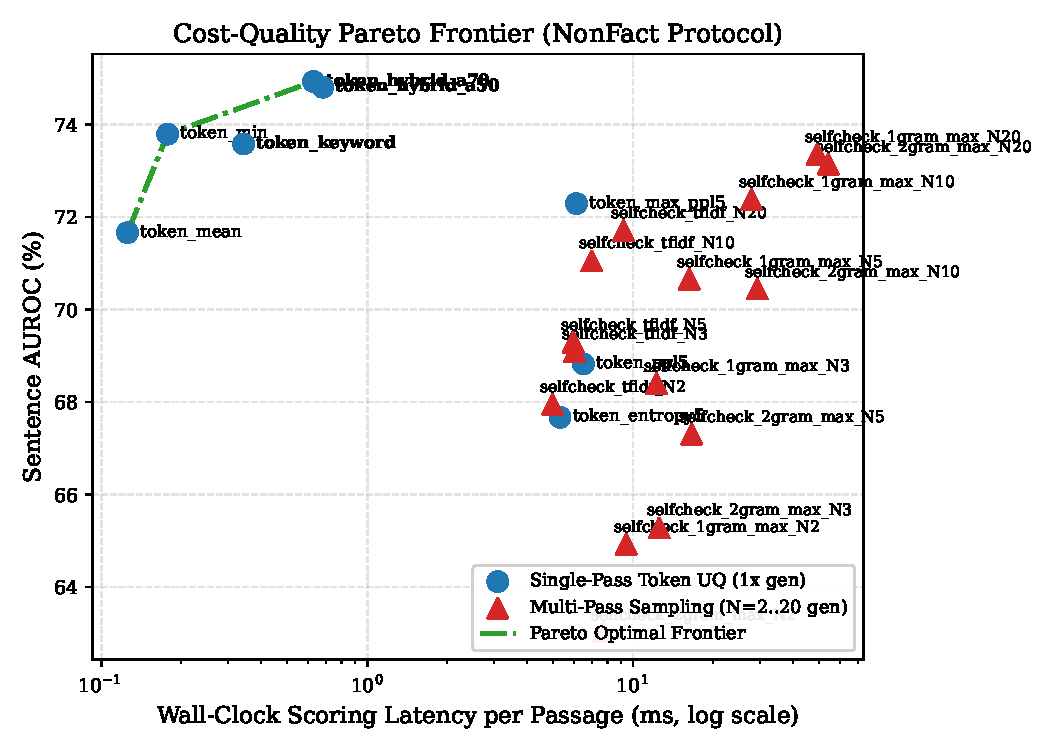
\includegraphics[width=0.98\linewidth]{fig3_pareto_frontier.pdf}
    \caption{The Cost-Quality Pareto Frontier on the \texttt{NonFact} benchmark. Single-pass methods define the Pareto-optimal frontier, dominating all multi-pass configurations with $N \le 5$.}
    \label{fig:pareto}
\end{figure}

\begin{figure}[t]
    \centering
    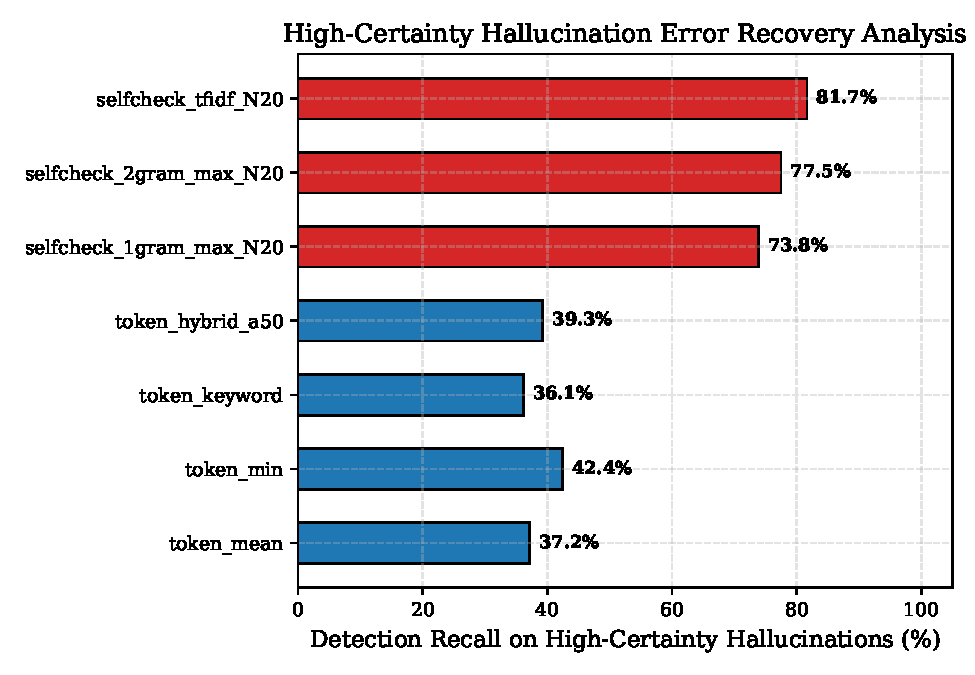
\includegraphics[width=0.98\linewidth]{fig4_high_certainty_breakdown.pdf}
    \caption{Detection recall on $N=191$ high-certainty hallucinations (bottom 25\% uncertainty of fabricated text). Single-pass token methods collapse ($<43\%$), whereas multi-pass consistency recovers up to $81.7\%$.}
    \label{fig:high_cert}
\end{figure}

\subsection{Deeper Analysis 1: The Cost-Quality Pareto Frontier}
Fig.~\ref{fig:pareto} maps the empirical Cost-Quality Pareto Frontier (Latency vs. AUROC). The frontier is exclusively bounded by:
\begin{enumerate}
    \item \texttt{token\_mean}: $0.13\text{ ms}$, $71.66\%$ AUROC (ultra-lightweight baseline).
    \item \texttt{token\_min}: $0.18\text{ ms}$, $73.79\%$ AUROC (fastest high-precision point).
    \item \texttt{token\_hybrid\_a70}: $0.63\text{ ms}$, $74.93\%$ AUROC (optimal single-pass point).
\end{enumerate}
All multi-pass configurations with $N \in \{2, 3, 5\}$ lie strictly beneath the single-pass Pareto hull, demonstrating that running few stochastic passes is a Pareto-suboptimal allocation of compute.

\subsection{Deeper Analysis 2: High-Certainty Hallucinations Autopsy (RQ3)}
To address \textbf{RQ3}, we examine the failure modes of uncertainty estimation on confident falsehoods. Following Simhi et al.~\cite{simhi2024high}, we isolate $N=191$ sentences labeled \texttt{major\_inaccurate} where \texttt{token\_mean} falls in the bottom quartile of uncertainty ($\le 0.3919$). We evaluate detection recall when each method operates at an $80\%$ global recall threshold.

As illustrated in Fig.~\ref{fig:high_cert}:
\begin{itemize}
    \item \texttt{token\_mean} detects only $71/191$ errors ($\mathbf{37.2\%}$ recall).
    \item \texttt{token\_keyword} detects $69/191$ errors ($\mathbf{36.1\%}$ recall).
    \item \texttt{token\_min} detects $81/191$ errors ($\mathbf{42.4\%}$ recall).
    \item \texttt{SelfCheck-1gram} ($N=20$) recovers $141/191$ errors ($\mathbf{73.8\%}$ recall, $+36.6\%$ gain).
    \item \texttt{SelfCheck-TFIDF} ($N=20$) recovers $156/191$ errors ($\mathbf{81.7\%}$ recall, $\mathbf{+44.5\%}$ gain).
\end{itemize}

This quantitative autopsy reveals an essential theoretical insight: \textbf{internal token uncertainty and external sampling consistency possess orthogonal failure boundaries.} When parametric memorization causes the model to hallucinate with extreme confidence, token probabilities fail. However, stochastic sampling exposes the hallucination because the model stochastically diverges across completions.

\subsection{Qualitative Case Study}
In Passage 0 (\textit{John Peter Russell}), the model generates: \textit{"He was educated at the Sydney Grammar School and then studied art at the Slade School of Fine Art in London."} (Annotated: \texttt{major\_inaccurate}). 

Because the Slade School is a high-frequency associate of Victorian painters in pre-training data, the model emits these tokens with high probability ($\text{token\_mean} = 0.392$), evading single-pass detection. However, across 20 stochastic samples, alternative generations cite the \textit{"Julian Academy"}, \textit{"Royal Academy"}, and \textit{"East London School"}. This cross-sample divergence yields a maximum TF-IDF inconsistency score of $0.960$, successfully intercepting the error.

\section{Limitations}
Our study possesses three primary limitations:
\begin{enumerate}
    \item \textbf{Dataset Scope:} Evaluation is conducted on the GPT-3 WikiBio biography benchmark. While biography generation is the canonical testbed for factual hallucination benchmarking~\cite{manakul2023selfcheckgpt, min2023factscore}, performance patterns may vary in multi-step reasoning or mathematical question-answering domains.
    \item \textbf{Model Access Constraints:} Our token features rely on grey-box access to top-5 output log-probabilities, which are standard in commercial APIs (e.g., OpenAI, Anthropic, Together AI). They do not extend to pure black-box interfaces where probabilities are entirely suppressed.
    \item \textbf{Static Fusion Weights:} The linear mixing parameter $\alpha=0.70$ in \texttt{token\_hybrid} was evaluated across fixed values without dynamic per-sentence adaptation.
\end{enumerate}

\section{Conclusion}
In this work, we resolved the operational tension between single-pass token uncertainty and multi-pass sampling consistency in LLM hallucination detection. We demonstrated that proposed single-pass methods (\texttt{token\_keyword} and \texttt{token\_hybrid}) establish a new state-of-the-art Pareto efficiency boundary, achieving $74.93\%$ AUROC at $0.63\text{ ms}$ latency and outperforming 20-sample SelfCheckGPT without additional inference passes. 

Simultaneously, our deep error analysis revealed that multi-pass consistency recovers over $81.7\%$ of high-certainty hallucinations that blind token-level detectors. We conclude that future trustworthy LLM architectures should adopt a two-tier hybrid paradigm: deploying lightweight single-pass token fusion as a real-time streaming gatekeeper, while conditionally routing borderline or high-stakes outputs to multi-pass consistency verification.

\bibliographystyle{IEEEtran}
\bibliography{references}

\end{document}
